\subsection{Loom}

В данном подразделе представлено подробное описание архитектуры и алгоритмов,
предложенных авторами в статье \cite{loom}. Изложение разбито на три
логические части, соответствующие основным этапам работы системы:
выявление частотных структур в нагрузке, обнаружение этих структур в потоке
графа и их размещение по разделам с учётом балансировки.

\subsubsection{Выявление мотивов запросов}

Первый этап работы Loom заключается в анализе заданного множества запросов
\( Q \) с целью выявления наиболее часто встречающихся подграфов, которые
авторы называют мотивами. Для этого предложена специализированная структура
данных --- TPSTry++ (Traversal Pattern Summary Trie), которая
представляет собой направленный ациклический граф, кодирующий все возможные
подграфы всех запросов из рабочей нагрузки.

\begin{figure}[h]
\centering
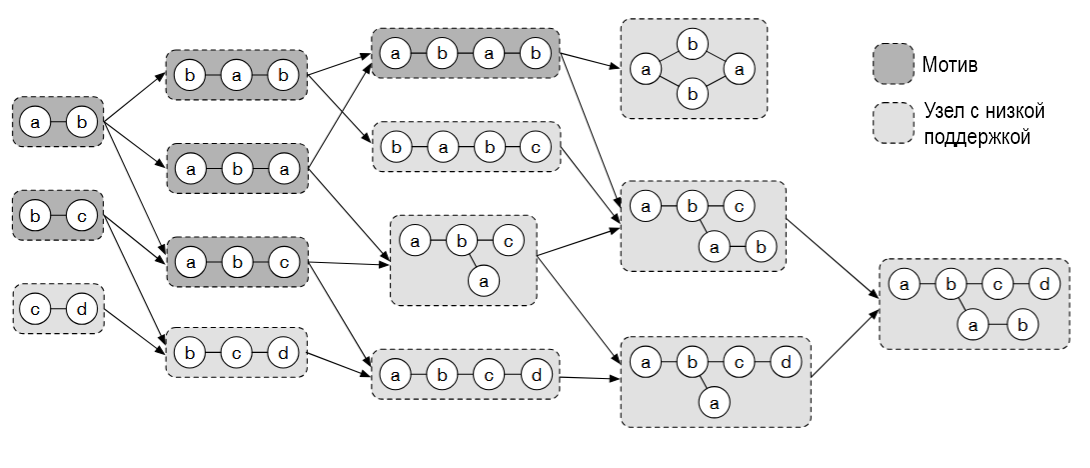
\includegraphics[width=0.8\textwidth]{extras/loom/motifs.png}
\caption{Пример структуры TPSTry++}
\label{fig:tptry}
\end{figure}

Каждый узел в TPSTry++ представляет собой уникальный подграф и хранит два
ключевых атрибута: его сигнатуру (компактное числовое представление) и значение
поддержки \(p\). Поддержка узла равна суммарной частоте вхождения данного
подграфа во все запросы из \( Q \). Мотивом считается любой узел, чья поддержка
превышает заданный порог \(\mathcal{T}\). Например, для порога
\(\mathcal{T} = 40\%\) мотивами будут все подграфы, встречающиеся более чем
в 40\% запросов.

Для эффективного сравнения подграфов и выявления изоморфизмов при построении
TPSTry++ авторы используют вероятностный метод, основанный на числовых
сигнатурах, расширяющий подход, предложенный в работе~\cite{song2014}.
Сигнатура графа \(G_q = (V_q, E_q)\) вычисляется следующим образом:
\begin{enumerate}
    \item Каждой метке вершины \(l \in L_V\) ставится в соответствие
    случайное простое число \(r(l)\) из диапазона \([1, p)\), где \(p\) ---
    заданное простое число.
    \item Для каждого ребра \(e = (v_i, v_j)\) вычисляется реберный фактор:
    \[
    \text{edgeFac}(e) = (r(f_l(v_i)) - r(f_l(v_j))) \mod p
    \]
    \item Для каждой вершины \(v\) со степенью \(n\) вычисляется фактор степени:
    \[
    \text{degFac}(v) = \prod_{k=1}^{n} ((r(f_l(v)) + k) \mod p)
    \]
    \item Итоговая сигнатура графа есть произведение всех реберных факторов и
    факторов степеней всех вершин:
    \[
    \text{sig}(G_q) = \left(\prod_{e \in E_q} \text{edgeFac}(e)\right) \cdot
    \left(\prod_{v \in V_q} \text{degFac}(v)\right)
    \]
\end{enumerate}

Ключевым преимуществом такого подхода является его инкрементальность.
Сигнатуру большего подграфа можно получить умножением сигнатуры меньшего
подграфа на факторы, соответствующие добавленным рёбрам и вершинам. Это
свойство активно используется на следующих этапах. Вероятность коллизий
(когда два неизоморфных графа имеют одинаковую сигнатуру) регулируется
выбором простого числа \(p\). Авторы показали, что при \(p = 251\)
вероятность коллизий для графов с числом рёбер до 16 является пренебрежимо
малой.

\subsubsection{Обнаружение мотивов в потоке обновлений графа}

Второй этап работы Loom выполняется в реальном времени по мере поступления
потока рёбер, формирующих динамический граф \(G\). Система поддерживает
скользящее окно фиксированного размера \(t\) (в рёбрах), которое служит
временным буфером. Новые рёбра сначала попадают в это окно, и лишь при
выходе из него окончательно распределяются по постоянным разделам.
Такая задержка позволяет накапливать контекст для принятия более взвешенных
решений о размещении. Само окно авторы рассматривают как временный раздел
\(P_{temp}\), что обеспечивает доступ к новым данным для запросов.

\begin{figure}[h]
\centering
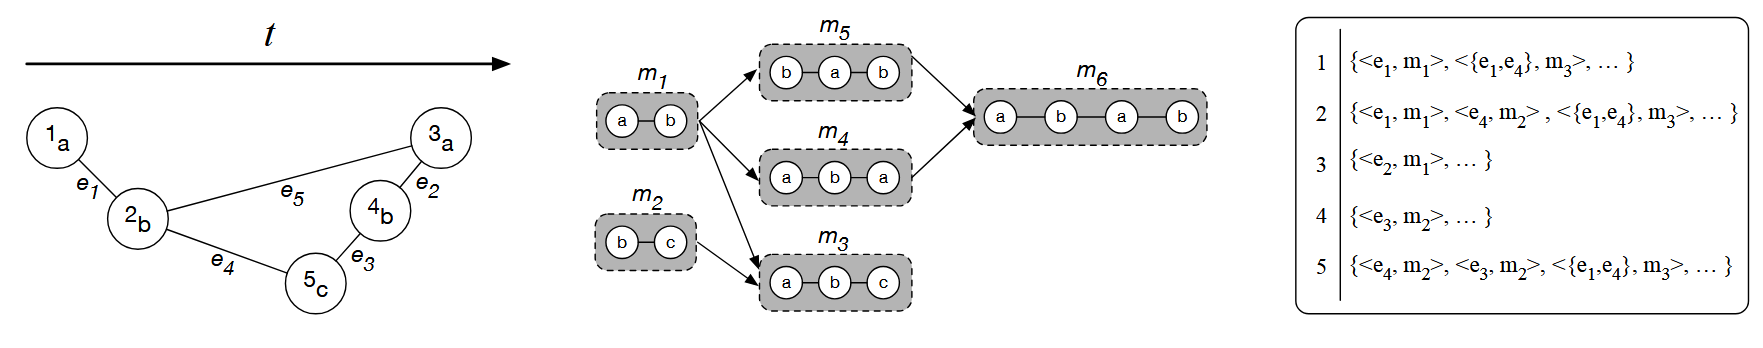
\includegraphics[width=1\textwidth]{extras/loom/matching.png}
\caption{Иллюстрация процесса сопоставления: Слева направо показаны: скользящее окно с рёбрами \(e_1...e_5\), набор мотивов из TPSTry++ (\(m_1...m_6\)) и содержимое matchList, где каждому мотиву сопоставлены обнаруженные подграфы.
}
\label{fig:matching}
\end{figure}

Процесс обнаружения мотивов в окне организован следующим образом:
\begin{enumerate}
    \item При поступлении нового ребра \(e = (v_1, v_2)\) вычисляется его
    сигнатура. Если она совпадает с сигнатурой однорёберного мотива в корне
    TPSTry++, ребро добавляется в окно \(P_{temp}\), а информация о новом
    совпадении заносится в структуру matchList. Эта структура
    отображает каждую вершину на множество обнаруженных мотивов, которым
    она принадлежит. Если ребро не совпадает ни с одним мотивом, оно
    немедленно распределяется в постоянный раздел, минуя окно.
    \item Если новое ребро инцидентно другим рёбрам, уже находящимся в окне,
    его добавление может привести к образованию более крупных подграфов,
    совпадающих с мотивами. Для проверки этого система использует matchList.
    Для каждого существующего подграфа \(g_i\), связанного с вершинами
    \(v_1\) или \(v_2\), вычисляются факторы \(\text{factors}(e, g_i)\),
    которые изменили бы его сигнатуру при добавлении \(e\).
    \item Затем проверяется, существует ли в TPSTry++ дочерний узел мотива,
    соответствующего \(g_i\), набор факторов которого отличается от
    родительского ровно на \(\text{factors}(e, g_i)\). Если такой узел
    существует и является мотивом, значит, новый подграф \(g_i + e\) также
    является мотивом, и это совпадение добавляется в matchList.
    \item Аналогичная проверка выполняется и для возможности объединения двух
    уже существующих в окне мотивов в один, более крупный, если они соединены
    через общую вершину.
\end{enumerate}

Благодаря такому подходу matchList всегда содержит актуальную информацию
обо всех подграфах в окне, которые являются мотивами, что служит основой
для принятия решений о распределении на следующем этапе.

\subsubsection{Размещение мотивов по разделам с учётом балансировки}

Заключительный этап алгоритма вступает в силу, когда окно \(P_{temp}\)
заполняется и новое ребро вытесняет из него самое старое ребро \(e\).
Именно в этот момент для ребра \(e\) и всех связанных с ним мотивов
принимается решение об окончательном размещении в одном из \(k\) постоянных
разделов \(S_i\). Цель --- разместить весь кластер рёбер, образующий мотив,
внутри одного раздела, минимизируя тем самым будущие межраздельные переходы.

Для достижения этой цели авторы предлагают комбинацию двух эвристик.
Для рёбер, не входящих в мотивы и потому не попавших в окно, применяется
известная эвристика LDG (Linear Deterministic Greedy)~\cite{SGP}.
Она назначает ребро в раздел \(S_i\), максимизируя взвешенную сумму:
\[
\max_{S_i\in P_k(G)} N(S_i, e) \cdot \left(1 - \frac{|\mathcal{V}(S_i)|}{C}\right),
\]
где \(N(S_i, e)\) --- число инцидентных ребру \(e\) вершин, уже находящихся
в разделе \(S_i\), \(\mathcal{V}(S_i)\) --- текущее число вершин в разделе,
а \(C\) --- ограничение на ёмкость раздела. Второй сомножитель играет роль
штрафа за переполнение, обеспечивая балансировку.

Для рёбер, которые являются частью мотивов и покидают окно, разработана
новая, более сложная эвристика Equal Opportunity. Пусть \(M_e\) ---
множество мотивов из matchList, содержащих ребро \(e\). Эвристика не просто
пытается разместить все эти мотивы в разделе с наибольшим числом общих вершин,
но делает это более избирательно, учитывая как поддержку самих мотивов, так
и необходимость глобальной балансировки.

Для каждого раздела \(S_i\) и каждого мотива \(\langle E_k, m_k \rangle \in M_e\)
вычисляется ставка (bid):
\[
\text{bid}(S_i,\langle E_k,m_k\rangle) = \mathcal{N}(S_i,E_k)\cdot
\left(1 - \frac{|\mathcal{V}(S_i)|}{C}\right)\cdot \text{supp}(m_k),
\]
где \(\mathcal{N}(S_i,E_k)\) --- количество вершин из множества рёбер \(E_k\),
уже принадлежащих разделу \(S_i\), а \(\text{supp}(m_k)\) --- поддержка мотива
\(m_k\) в TPSTry++.

Ключевым нововведением является использование рационирующей функции
\(l(S_i)\). Эта функция ограничивает "жадность" алгоритма, определяя, какая
часть мотивов из \(M_e\) будет участвовать в формировании итоговой ставки
для раздела \(S_i\) и, в случае его победы, какая часть будет ему назначена.
\(l(S_i)\) вычисляется на основе относительного размера раздела:
\[
l(S_i) = \frac{|\mathcal{V}(S_i)|}{\min_{S \in P_k(G)} |\mathcal{V}(S)|} \cdot \alpha,
\]
где \(\alpha\) --- параметр, управляющий агрессивностью рационирования
(авторы используют \(\alpha = 2/3\)). Функция устроена так, что меньшие
разделы получают большее значение \(l(S_i)\) и, следовательно, могут
участвовать в торгах за большее число мотивов, что способствует выравниванию
нагрузки.

Итоговое решение о размещении принимается на основе максимизации суммы ставок
по первым \(l(S_i) \cdot |M_e|\) мотивам в множестве \(M_e\), отсортированным
по убыванию поддержки \(\text{supp}(m_k)\):
\[
\max_{S_i\in P_k(G)} \sum_{k = 0}^{l(S_i)\cdot |M_e|} \text{bid}(S_i,\langle E_k,m_k\rangle).
\]

Такой подход гарантирует, что:
\begin{itemize}
    \item Мотивы с наивысшей поддержкой (наиболее часто встречающиеся в
    запросах) имеют приоритет при размещении.
    \item Уже переполненные разделы ограничены в возможности получить новые,
    даже очень "ценные", кластеры рёбер, что сохраняет общий баланс системы.
    \item Рёбра, которые не были назначены победившему разделу, остаются в
    окне \(P_{temp}\), получая шанс быть назначенными позже вместе с другими,
    более релевантными для них мотивами.
\end{itemize}

\subsubsection{Оценка эффективности}
\label{sec:evaluation-summary}

В ходе экспериментальной оценки авторы сравнили Loom с хешированием (baseline),
а также с потоковыми партиционерами LDG и Fennel \cite{Fennel}. В качестве основной метрики
качества использовалось количество межраздельных переходов (IPT) при выполнении
реалистичной нагрузки запросов на разделах, построенных каждым из методов.

\begin{table}[h]
\centering
\small
\setlength{\tabcolsep}{4pt}
\begin{tabularx}{\textwidth}{|l|X|c|c|}
\hline
\textbf{Метод} & \textbf{IPT (отн. Hash)} & \textbf{Скорость (рёбер/с)} & \textbf{Зависимость от порядка} \\
\hline
Hash & 100\% (базовый уровень) & --- & Нет \\
LDG & \(\approx 45\%\) & \(\approx 100\)k & Средняя \\
Fennel & \(\approx 20\)-\(25\%\) (лучше LDG) & \(\approx 70\)k & Средняя \\
Loom & \(15\)-\(40\%\) (лучше Fennel) & \(\approx 42\)-\(72\)k & Высокая \\
\hline
\end{tabularx}
\caption{Сравнительная эффективность алгоритмов распределения. \cite{loom}}
\label{tab:comparison}
\end{table}

Результаты, обобщённые в Таблице~\ref{tab:comparison}, демонстрируют
значительное превосходство Loom над существующими решениями:
\begin{itemize}
    \item Loom стабильно обеспечивает на 20–25\% меньшее количество
    межраздельных переходов по сравнению с Fennel, который является лучшим
    из workload-agnostic алгоритмов. В отдельных случаях, например, на
    гетерогенном графе MusicBrainz при BFS-порядке поступления данных,
    улучшение достигало 42\%.
    \item Преимущество сохраняется для различного количества разделов (от 2 до 32).
    \item Основная плата за повышение качества --- чувствительность к порядку
    поступления данных (особенно к случайному) и некоторое снижение скорости
    работы (в 2-3 раза медленнее Fennel). Однако даже в медленном режиме
    Loom обрабатывает более 40 000 рёбер в секунду, что, по мнению авторов,
    достаточно для большинства практических онлайн-сценариев.
    \item Увеличение размера скользящего окна позволяет значительно снизить
    негативное влияние случайного порядка поступления.
\end{itemize}

Таким образом, предложенное решение Loom успешно демонстрирует применимость
и высокую эффективность подхода, учитывающего информацию о запросах при
потоковом распределении динамических графов.